% !TeX spellcheck = <none>
\documentclass{article}
\usepackage{graphicx}
\usepackage{pdfpages}

\usepackage{amsmath}
\usepackage{listings}
\usepackage{color} %red, green, blue, yellow, cyan, magenta, black, white
\definecolor{mygreen}{RGB}{28,172,0} % color values Red, Green, Blue
\definecolor{mylilas}{RGB}{170,55,241}


\begin{document}
	\lstset{language=Matlab,%
		%basicstyle=\color{red},
		breaklines=true,%
		morekeywords={matlab2tikz},
		keywordstyle=\color{blue},%
		morekeywords=[2]{1}, keywordstyle=[2]{\color{black}},
		identifierstyle=\color{black},%
		stringstyle=\color{mylilas},
		commentstyle=\color{mygreen},%
		showstringspaces=false,%without this there will be a symbol in the places where there is a space
		numbers=left,%
		numberstyle={\tiny \color{black}},% size of the numbers
		numbersep=9pt, % this defines how far the numbers are from the text
		emph=[1]{for,end,break},emphstyle=[1]\color{red}, %some words to emphasise
		%emph=[2]{word1,word2}, emphstyle=[2]{style},    
	}
	
	\begin{center}
		\Large\textbf{CS3081: Computational Maths}\\
		\large\textit{Owen Burke (15316452) : Assignment Three}
	\end{center}
	\section{\normalsize{4.26 Write a user-defined MATLAB function that calculates the infinity norm of any matrix. For the func­ tion name and arguments use N = InfinityNorm (A), where A is the matrix, and N is the value of the norm. Use the function for calculating the infinity norm of:}}
		$${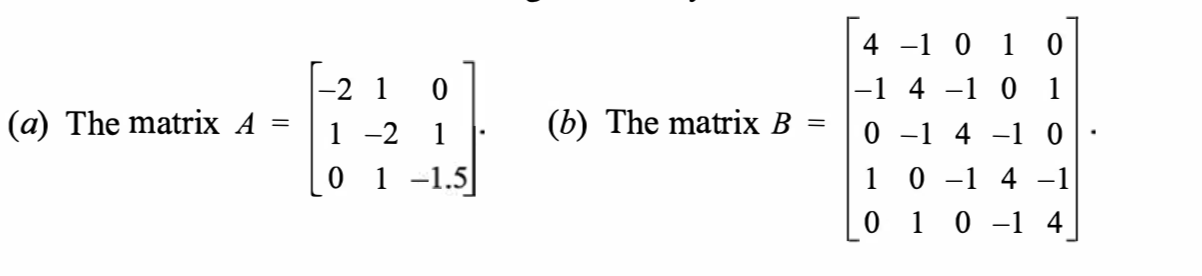
\includegraphics[width=12cm]{matAB.png}}$$
		
		\subsection*{}
		The infinity norm of a matrix is simply given as the maximum of the sums of the rows of the matrix where the 
		values used are the absolute values of the elements in the matrix.(See the matlab code below)
		
		\lstinputlisting{InfinityNorm.m}
		
		The following images show the answers to the question, shown in matlab.
		
		\begin{figure}[h!]
			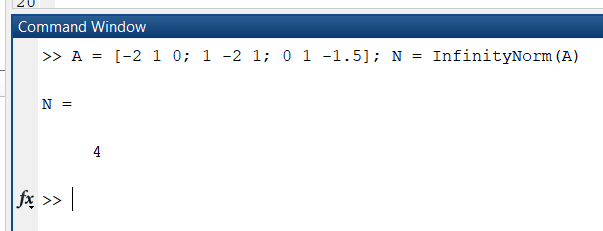
\includegraphics[width=\linewidth]{oneA.png}
			\caption{InfinityNorm for a}
			\label{fig:InfinityNorm_a}
		\end{figure}
	
		\begin{figure}[h!]
			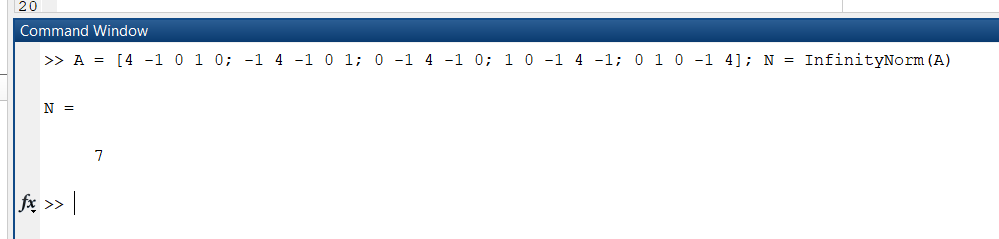
\includegraphics[width=\linewidth]{oneB.png}
			\caption{InfinityNorm for a}
			\label{fig:InfinityNorm_a}
		\end{figure}
		
		
		
	\newpage
	
	\section{The power generated by a windmill varies with the wind speed. In an experiment, the following five measurements were obtained:}

			$${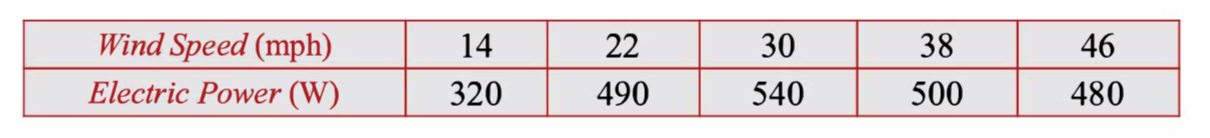
\includegraphics[width=12cm]{table.png}}$$
	
	\subsection*{Determine the fourth-order polynomial in the Lagrange form that passes through the points. Use the polynomial to calculate the power at a wind speed of 26 mph.}
	
	\subsection*{}
	Given points :\\
	(X$_1$, Y$_1$) = (14, 320)\\
	(X$_2$, Y$_2$) = (22, 490)\\
	(X$_3$, Y$_3$) = (30, 540)\\
	(X$_4$, Y$_4$) = (38, 500)\\
	(X$_5$, Y$_5$) = (46, 480)\\
	
	And given that we know the form of a lagrange polynomial that passes through five points is given as\\
	
	y = f(x) = $\frac{(X - X_2)(X - X_3)(X - X_4)(X - X_5)}{(X_1 - X_2)(X_1 - X_3)(X_1 - X_4)(X_1 - X_5)}$Y$_1$ + 
	$\frac{(X - X_1)(X - X_3)(X - X_4)(X - X_5)}{(X_2 - X_1)(X_2 - X_3)(X_2 - X_4)(X_2 - X_5)}$Y$_2$ + 
	$\frac{(X - X_1)(X - X_2)(X - X_4)(X - X_5)}{(X_3 - X_1)(X_3 - X_2)(X_3 - X_4)(X_3 - X_5)}$Y$_3$ + 
	$\frac{(X - X_1)(X - X_2)(X - X_3)(X - X_5)}{(X_4 - X_1)(X_4 - X_2)(X_4 - X_3)(X_4 - X_5)}$Y$_4$ + 
	$\frac{(X - X_1)(X - X_2)(X - X_3)(X - X_4)}{(X_5 - X_1)(X_5 - X_2)(X_5 - X_3)(X_5 - X_4)}$Y$_5$\\\\
	
	The Y$_1$ part of the above equation (given the points from the question) gives\\\\
	($\frac{(X - 22)(X - 30)(X - 38)(X - 46)}{(14 - 22)(14 - 30)(14 - 38)(14 - 46)}$)(320)\\\\
	which gives \\\\
	($\frac{x^4 - 136x^3 + 6776x^2 - 146336x + 1153680}{98304}$)(320)\\\\
	
	The Y$_2$ part of the above equation (given the points from the question) gives\\\\
	($\frac{(X - 14)(X - 30)(X - 38)(X - 46)}{(22 - 14)(22 - 30)(22 - 38)(22 - 46)}$)(490)\\\\
	which gives \\\\
	($\frac{x^4 - 128x^3 + 5864x^2 - 112192x + 734160}{-24576}$)(490)\\\\
	
	The Y$_3$ part of the above equation (given the points from the question) gives\\\\
	($\frac{(X - 14)(X - 22)(X - 38)(X - 46)}{(30 - 14)(30 - 22)(30 - 38)(30 - 46)}$)(540)\\\\
	which gives \\\\
	($\frac{x^4 - 120x^3 + 5080x^2 - 88800x + 538384}{16384}$)(540)\\\\
	
	The Y$_4$ part of the above equation (given the points from the question) gives\\\\
	($\frac{(X - 14)(X - 22)(X - 30)(X - 46)}{(38 - 14)(38 - 22)(38 - 30)(38 - 46)}$)(500)\\\\
	which gives \\\\
	($\frac{x^4 - 112x^3 + 4424x^2 - 73088x + 425040}{-24576}$)(500)\\\\
	
	The Y$_5$ part of the above equation (given the points from the question) gives\\\\
	($\frac{(X - 14)(X - 22)(X - 30)(X - 38)}{(46 - 14)(46 - 22)(46 - 30)(46 - 38)}$)(480)\\\\
	which gives \\\\
	($\frac{x^4 - 104x^3 + 3896x^2 - 61984x + 351120}{98304}$)(480)\\\\\\
	
	All this gives :\\\\
	y = f(x) = ($\frac{x^4 - 136x^3 + 6776x^2 - 146336x + 1153680}{98304}$)(320) + ($\frac{x^4 - 128x^3 + 5864x^2 - 112192x + 734160}{-24576}$)(490) + ($\frac{x^4 - 120x^3 + 5080x^2 - 88800x + 538384}{16384}$)(540) + ($\frac{x^4 - 112x^3 + 4424x^2 - 73088x + 425040}{-24576}$)(500) + ($\frac{x^4 - 104x^3 + 3896x^2 - 61984x + 351120}{98304}$)(480)\\\\
	
	For a wind speed of 26 mph, simply substitute 26 in for x, giving :\\\\
	f(26) = -12$\frac{1}{2}$ + 229$\frac{11}{16}$ + 379$\frac{11}{16}$ - 78$\frac{1}{8}$ + 11$\frac{1}{4}$\\\\
	giving \\\\
	f(26) = 530 W
	
	
	
	
	
	
	
	
	\newpage
			\section{Derive a finite difference approximation formula for f"($x_{i}$) using three points $x_{i-1}$, x, and $x_{i+1}$, where the spacing is such that $x_i - x_{i-1} = 2h $ and $x_{i+1} - x_{i} = h $}
			$${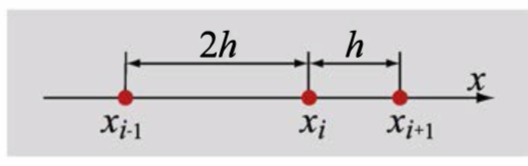
\includegraphics[width=12cm]{points.png}}$$
			
			
	\subsection*{}
	From the above diagram and from the taylor series, we can obtain the following equations :\\\\
	f(x$_{i+1}$) = f(x$_i$) + f$'$(x$_i$)h + $\frac{f''(x_i)}{2!}$h$^2$ + $\frac{f'''(x_i)}{3!}$h$^3$ + $\frac{f^{(4)}(\epsilon_1)}{4!}$h$^4$ \\
	
	and \\
	
	f(x$_{i-1}$) = f(x$_i$) - f$'$(x$_i$)2h + $\frac{f''(x_i)}{2!}$(2h)$^2$ - $\frac{f'''(x_i)}{3!}$(2h)$^3$ + $\frac{f^{(4)}(\epsilon_2)}{4!}$(2h)$^4$ \\
	
	f(x$_{i-1}$) simplifies down to : \\
	
	f(x$_{i-1}$) = f(x$_i$) - 2f$'$(x$_i$)h + 4$\frac{f''(x_i)}{2!}$h$^2$ - 8$\frac{f'''(x_i)}{3!}$h$^3$ + 16$\frac{f^{(4)}(\epsilon_2)}{4!}$h$^4$ \\
	
	In order to obtain our desired equation, we need to cancel unwanted terms. However, if we now add the two equations above, some terms won't cancel, so we multiply f(x$_{i+1}$) by 2, giving :\\
	
	2f(x$_{i+1}$) = 2f(x$_i$) + 2f$'$(x$_i$)h + 2$\frac{f''(x_i)}{2!}$h$^2$ + 2$\frac{f'''(x_i)}{3!}$h$^3$ + 2$\frac{f^{(4)}(\epsilon_1)}{4!}$h$^4$ \\
	
	Now we get f(x$_{i-1}$) + 2f(x$_{i+1}$) as :\\
	f(x$_{i-1}$) + 2f(x$_{i+1}$) = 3f(x$_i$) + 3f$''$(x$_i$)h$^2$ + f$'''$(x$_i$)h$^3$ + 2$\frac{f^{(4)}(\epsilon_1)}{4!}$h$^4$ + 16$\frac{f^{(4)}(\epsilon_2)}{4!}$h$^4$\\\\
	
	We can now solve for f$''(x_i)$, as : \\
	
	f(x$_{i-1}$) + 2f(x$_{i+1}$) = 3f(x$_i$) + 3f$''$(x$_i$)h$^2$ + f$'''$(x$_i$)h$^3$ + 2$\frac{f^{(4)}(\epsilon_1)}{4!}$h$^4$ + 16$\frac{f^{(4)}(\epsilon_2)}{4!}$h$^4$ \\\\
	
	f(x$_{i-1}$) + 2f(x$_{i+1}$) - 3f(x$_i$) = 3f$''$(x$_i$)h$^2$ + f$'''$(x$_i$)h$^3$ + 2$\frac{f^{(4)}(\epsilon_1)}{4!}$h$^4$ + 16$\frac{f^{(4)}(\epsilon_2)}{4!}$h$^4$ \\
	
	Now divide across by 3h$^2$ to isolate f$''$ : \\
	
	$\frac{f(x_{i-1}) + 2f(x_{i+1}) - 3f(x_i)}{3h^2}$ = f$''$(x$_i$) + $\frac{f'''(x_i)h}{3}$ + (2$\frac{f^{(4)}(\epsilon_1)}{4!}$h$^4$)/(3h$^2$) + (16$\frac{f^{(4)}(\epsilon_2)}{4!}$h$^4$)/(3h$^2$) \\
	
	After truncating from f$'''$ and the higher terms, we get :\\
	
	f$''$(x$_i$) = $\frac{f(x_{i-1}) + 2f(x_{i+1}) - 3f(x_i)}{3h^2}$ + O(h)
	
	
	
	
	
	
	
	
	
	
	
	
			
			
			
	\newpage
	\section{The following data show the number of female and male physicians in the U.S. for various years (American Medical Association):}
	$${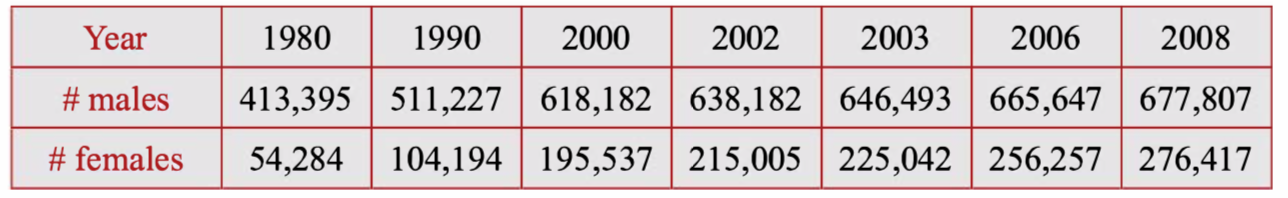
\includegraphics[width=12cm]{medicalTable.png}}$$
	\subsection{(a) Calculate the rate of change in the number of male and female physicians in 2006 by using the three­ point backward difference formula for the derivative, with unequally spaced points}
	
	\subsection{(b) Use the result from part (a) and the three-point central difference formula for the derivative with unequally spaced points, Eq. (8.36), to calculate (predict) the number of male and female physicians in 2008.}
	
	
	\subsection*{(a)}
	By using the three point backward difference formula for the derivative, with unequally spaced points, Eq.(8.37)
	given as :\\\\
	f'(x\textsubscript{i+2}) = $\frac{x\textsubscript{i+2} - x\textsubscript{i+1}}{(x_i - x\textsubscript{i+1})
		(x_i - x\textsubscript{i+2})}$y$_i$
	+
	$\frac{x\textsubscript{i+2} - x\textsubscript{i}}{(x\textsubscript{i+1} - x\textsubscript{i})
		(x\textsubscript{i+1} - x\textsubscript{i+2})}$y\textsubscript{i+1}
	+
	$\frac{2x\textsubscript{i+2} - x\textsubscript{i} - x\textsubscript{i+1}}{(x\textsubscript{i+2} - x\textsubscript{i})
		(x\textsubscript{i+2} - x\textsubscript{i+1})}$y\textsubscript{i+2}\\\\
	
	and taking x\textsubscript{i+2} = 2006, x\textsubscript{i+1} = 2003 and x\textsubscript{i} = 2002, we simply sub in the corresponding y values for the men and women.\\\\
	The men values give the following :\\\\
	
	f'(2006) = $\frac{2006 - 2003}{(2002-2003)(2002-2006)}$(638182)
	+
	$\frac{2006 - 2002}{(2003-2002)(2003-2006)}$(646493)
	+
	$\frac{2(2006) - 2002 - 2003}{(2006-2002)(2006-2003)}$(665647) = 4939.916633\\\\
	
	The women values give the following :\\\\
	
	f'(2006) = $\frac{2006 - 2003}{(2002-2003)(2002-2006)}$(215005)
	+
	$\frac{2006 - 2002}{(2003-2002)(2003-2006)}$(225042)
	+
	$\frac{2(2006) - 2002 - 2003}{(2006-2002)(2006-2003)}$(256257) = 10681\\\\
	
	\subsection*{(b)}
	By using the three point central difference formula for the derivative with unequally spaced points, Eq.(8.36) given as :\\\\
	
	f'(x\textsubscript{i+1}) = $\frac{x\textsubscript{i+1} - x\textsubscript{i+2}}{(x_i - x\textsubscript{i+1})
		(x_i - x\textsubscript{i+2})}$y$_i$
	+
	$\frac{2x\textsubscript{i+1} - x\textsubscript{i} - x\textsubscript{i+2}}{(x\textsubscript{i+1} - x\textsubscript{i})
		(x\textsubscript{i+1} - x\textsubscript{i+2})}$y\textsubscript{i+1}
	+
	$\frac{x\textsubscript{i+1} - x\textsubscript{i}}{(x\textsubscript{i+2} - x\textsubscript{i})
		(x\textsubscript{i+2} - x\textsubscript{i+1})}$y\textsubscript{i+2}\\\\
	
	and taking x\textsubscript{i+2} = 2008, x\textsubscript{i+1} = 2006 and x\textsubscript{i} = 2003, we simply sub in the corresponding y values for the men and women and solve for the unknown to predict the number of physicians in 2008, as we know f'(2006) from part a.\\\\
	The men values give the following :\\\\
	
	4940 = $\frac{2006 - 2008}{(2003-2006)(2003-2008)}$(646493)
	+
	$\frac{2(2006) - 2003 - 2008}{(2006-2003)(2006-2008)}$(665647)
	+
	$\frac{2006 - 2003}{(2008-2003)(2008-2006)}$(a)\\\\

	This gives :\\\\
	4940 = (-86199$\frac{1}{15}$) + (-110941$\frac{1}{6}$) + $\frac{3}{10}$a\\
	202080.2333 = $\frac{3}{10}$a\\
	a = 673600$\frac{7}{9}$ = predicted male physicians in 2008\\
	error = 100 - ($\frac{673600\frac{7}{9}}{677807}$ * 100) = 0.62056\\\\
	
	
	The women values give the following :\\\\
	
	10681 = $\frac{2006 - 2008}{(2003-2006)(2003-2008)}$(225042)
	+
	$\frac{2(2006) - 2003 - 2008}{(2006-2003)(2006-2008)}$(256257)
	+
	$\frac{2006 - 2003}{(2008-2003)(2008-2006)}$(a)\\\\
	
	This gives :\\\\
	10681 = (-30005$\frac{3}{5}$) + (-42709$\frac{1}{2}$) + $\frac{3}{10}$a\\
	83396$\frac{1}{10}$ = $\frac{3}{10}$a\\
	a = 277987 = predicted female physicians in 2008\\
	error = 100 - ($\frac{276417}{277987}$ * 100) = 0.56477\\\\
	
	
	
	
	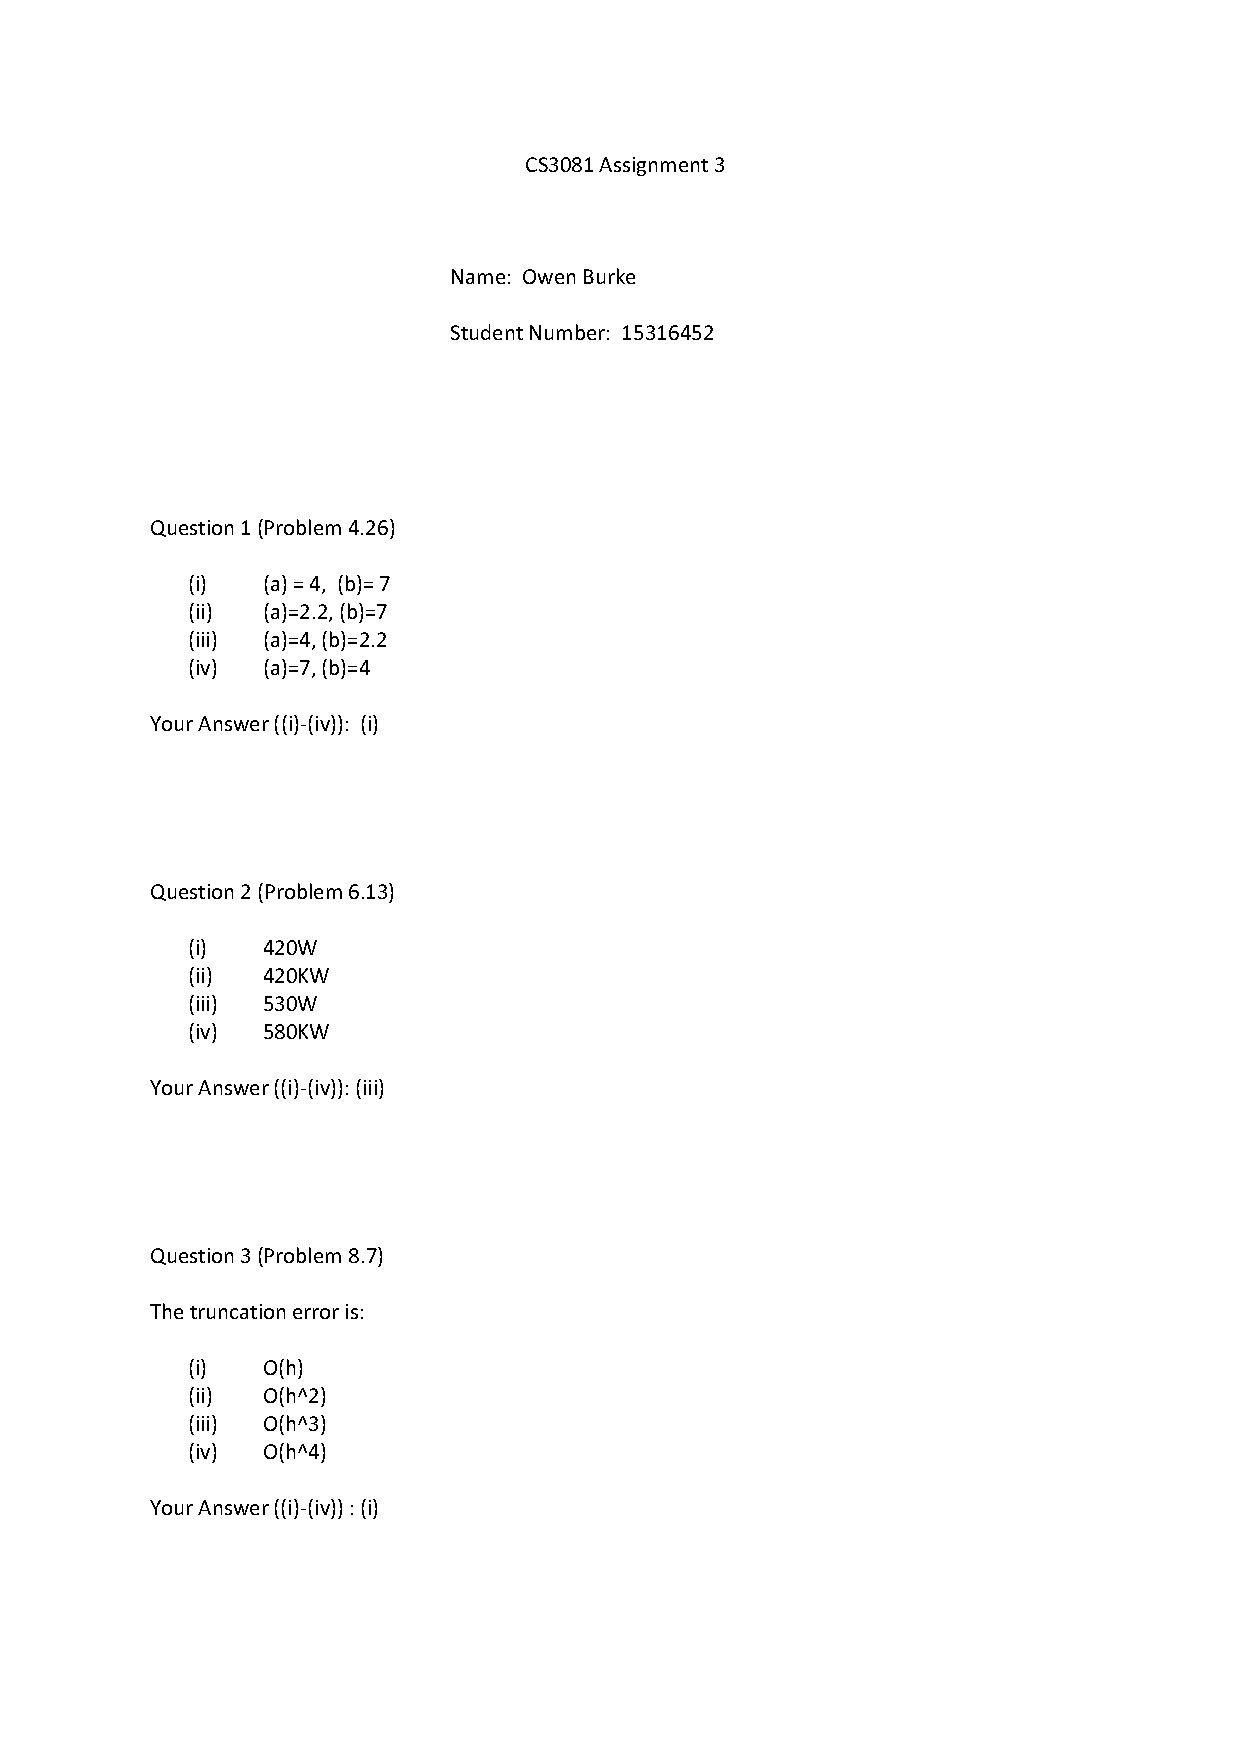
\includepdf[page=-]{Assignment3_multichoice.pdf}
	
	
	
				
\end{document}